\documentclass{article}
\usepackage[utf8]{inputenc}
\usepackage{amsmath}
\usepackage{amssymb}
\usepackage{mathtools}
\usepackage{graphicx}

\graphicspath{{Images/}}

\setlength{\oddsidemargin}{0in}
\setlength{\textwidth}{6.5in}
\setlength{\topmargin}{-.55in}
\setlength{\textheight}{9in}
\pagestyle{empty}



\title{Solid State Physics HW 7}
\author{Michael Nameika}
\date{November 2022}

\begin{document}

\maketitle

\section*{Problem 1}
Consider transverse vibrations of a square lattice with a distance between nn atoms to be "a". All atoms and force constants are equal (mass M and force constant C respectively). Find the equation of motion for nearest neighbor coupling and determine the dispersion relations. Determine the first Brillouin zone. What is the maximum magnitude of the k vector? Draw 6 equipotential lines (k-points with equal energy), approximately evenly spaced between a minimum and maximum values of k.
\newline\newline
See attached sketch for details on the equations of motion on the square lattice. We have that the maximum allowed values for $k$ are $k = \pm\frac{\pi}{a}$ and so the first Brillouin zone is the region in $\mathbb{R}^2$ given by $\left[-\frac{\pi}{a},\frac{\pi}{a}\right] \times \left[-\frac{\pi}{a},\frac{\pi}{a}\right]$. The equation of motion for nearest neighbor coupling is given by
\[M\frac{d^2u_{m,n}}{dt^2} = C[u_{m+1,n} + u_{m-1,n} + u_{m,n+1} + u_{m,n-1} - 4u_{n,m}]\]
We seek traveling wave solutions of the form
\[u_{m,n} = u_0e^{i(mk_xa + nk_ya - \omega t)}\]
Then substituting this into our equation of motion, we find
\begin{align*}
    -\omega^2M &= C\left[e^{ik_xa}+e^{-1k_xa} + e^{ik_ya} + e^{-ik_ya} - 4\right] \\
    &= \left[2\cos{(k_xa)} + 2\cos{(k_ya)} - 4\right] \\
    \omega^2 &= \frac{2C}{M}\left[(1-\cos{(k_xa)}) + (1-\cos{(k_ya)})\right] \\
    &= \frac{4C}{M}\left[\sin^2{\left(\frac{1}{2}k_xa\right)} + \sin^2{\left(\frac{1}{2}k_ya\right)}\right] \\
    \omega &= \pm\sqrt{\frac{4C}{M}}\left[\sin^2{\left(\frac{1}{2}k_xa\right)} + \sin^2{\left(\frac{1}{2}k_ya\right)}\right]^{1/2}\\
\end{align*}
And finally, below is a plot for 6 equipotential curves:
\begin{center}
    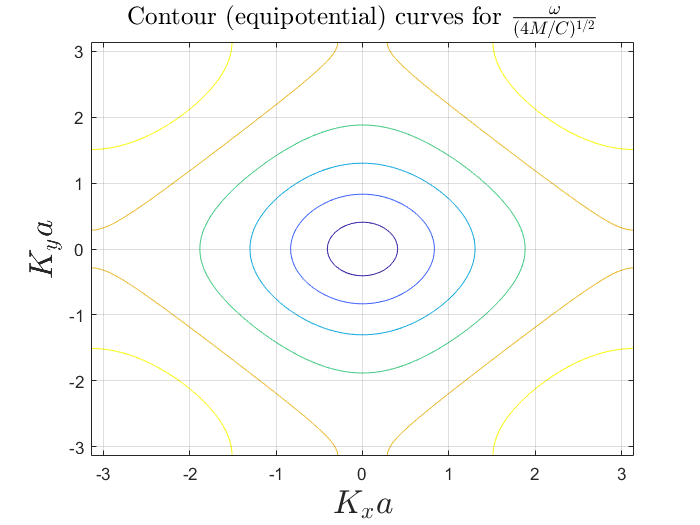
\includegraphics[scale = 0.6]{equipotentialcurves.png}
\end{center}


\section*{Problem 5.1} \textbf{\textit{Singularity in density of states.}} (a) From the dispersion relation derived in Chapter 4 for a monatomic linear lattice of $N$ atoms with nearest-neighbor interactions, show that the density of modes is
\[\mathcal{D}(\omega) = \frac{2N}{\pi}\frac{1}{(\omega_m^2 - \omega^2)^{1/2}}\]
where $\omega_m$ is the maximum frequency.
\newline\newline
Recall from Chapter 4 that the dispersion relation for a monatomic linear lattice of $N$ atoms is given by
\[\omega = \sqrt{\frac{4C}{M}}\sin^2{(1/2Ka)}\]
Clearly, from the above equation, we have $\omega_m = 4C/M$. Solving this equation for $K$, we find
\begin{align*}
    K &= \frac{2}{a}\arcsin{\left(\frac{\omega}{\omega_m}\right)} \\
\end{align*}
Then
\begin{align*}
    \frac{dK}{d\omega} &= \frac{2}{a}\left(\frac{1}{(1 - \omega^2/\omega_m^2)^{1/2}}\right)\left(\frac{1}{\omega_m}\right) \\
    &= \frac{2}{a}\frac{1}{(\omega_m^2 - \omega^2)^{1/2}} \\
\end{align*}
Then our density of states takes the form
\begin{align*}
    \mathcal{D}(\omega) &= \frac{2L}{\pi a}\frac{1}{(\omega_m^2 - \omega^2)^{1/2}} \\
\end{align*}
And since $L = Na$ for a linear lattice, we have
\[\mathcal{D}(\omega) = \frac{2N}{\pi}\frac{1}{(\omega_m^2 - \omega^2)^{1/2}}\]
Which is what we wanted to show.
\newline\newline
(b) Suppose that an optical phonon branch form $\omega(K) = \omega_0 - AK^2$, near $K = 0$ in three dimensions. Show that $\mathcal{D}(\omega) = (L/(2\pi))^3(2\pi/A^{3/2})(\omega_0 - \omega)^{1/2}$ for $\omega < \omega_0$ and $\mathcal{D}(\omega) = 0$ for $\omega > \omega_0$. Here the density of modes is discontinuous.
\newline\newline
To begin, suppose that $\omega < \omega_0$ and recall that for a three dimensional cubic lattice that 
\[\mathcal{D}(\omega) = \frac{\partial N}{\partial \omega}\]
and 
\[N = \frac{4\pi}{3}K^3\left(\frac{L}{2\pi}\right)^3\]
Thus,
\begin{align*}
    \frac{\partial N}{\partial \omega} &= 4\pi K^2\frac{\partial K}{\partial \omega}\left(\frac{L}{2\pi}\right)^3 \\
    \frac{\partial K}{\partial \omega} &= \frac{\partial}{\partial \omega} \left(\frac{\omega_0 - \omega}{A}\right)^{1/2} \\
    &= -\frac{1}{2A^{1/2}(\omega_0 - \omega)^{1/2}} \\
\end{align*}
so 
\begin{align*}
    \frac{\partial N}{\partial \omega} &= 4\pi\left(\frac{L}{2\pi}\right)^3\frac{\omega_0 - \omega}{A}\frac{-1}{2A^{1/2}(\omega_0 - \omega)^{1/2}} \\
    &= \left(\frac{L}{2\pi}\right)^3\left(\frac{2\pi}{A^{3/2}}\right)\frac{\omega_0 - \omega}{(\omega_0 - \omega)^{1/2}} \\
    &= \left(\frac{L}{2\pi}\right)^3\left(\frac{2\pi}{A^{3/2}}\right)(\omega_0 -\omega)^{1/2} \\
\end{align*}
Thus $\mathcal{D}(\omega) = (L/2\pi)^3(2\pi/A^{3/2})(\omega_0 - \omega)^{1/2}$ which is what we wished to show.
\newline\newline

\section*{Problem 5.2} \textbf{\textit{Rms thermal dilation of crystal cell.}} (a) Estimate for 300 K the root mean square thermal dilation $\Delta V/V$ for a primitive cell of sodium. Take the bulk modulus as $7 \times 10^{10} \text{ erg cm}^{-3}$. Note that the Debye temperature 158 K is less than 300 K, so that the thermal energy is of the order of $k_BT$. 
\newline\newline
Recall that $U_{thermal} = \frac{1}{2}B\delta^2a^3$ where $\delta \equiv \Delta V/V$. We also have that $U_{thermal} = \frac{1}{2}k_bT$, so we have
\[\frac{1}{2}B\left(\frac{\Delta V}{V}\right)^2a^3 = \frac{1}{2}k_bT\]
Solving, we have
\[\frac{\Delta V}{V} = \sqrt{\frac{k_bT}{Ba^3}}\]
Using $k_b = 1.38062 \times 10^{-16} \text{ erg }K^{-1}$, we find
\[\frac{\Delta V}{V} \approx 0.0886\]
\newline\newline
(b) Use this result to estimate the root mean square thermal fluctuation $\Delta a/a$ of the lattice parameter.
\newline\newline
In the limit where $\Delta V$ is "small", we have $\Delta V/V = 3\Delta a/a$, so from part (a), we find
\[\frac{\Delta a}{a} \approx 0.02953\]

\section*{Problem 4}
Gr{\"u}neisen Parameter. Calculate the Gr{\"u}neisen parameter, $\gamma = -d\ln{(\omega)}/d\ln{(L)}$, for a linear chain of length L, lattice spacing a, and only nearest-neighbor interaction. Assume that the interaction potential has a form of $U(x) = U_0 + 0.5\kappa x^2 + \lambda x^3$, where $x = d - a$, and $d$ is the distance between nearest neighbors.
\newline\newline
To begin, recall that the maximum frequency for the equation of motion for a linear lattice is given by $\omega_m = \sqrt{4C/M}$. For us, our force constant is given by $C = F = -dU/dx = -\kappa x - 3\lambda x^2$. Rewriting, we see
\[F = -x(\kappa + 3\lambda x^2)\]
which is of the form of Hooke's law with spring (force) constant $\kappa + 3\lambda x^2$. Thus $\omega_m$ takes the form
\[\omega_m = \sqrt{\frac{4(\kappa + 3\lambda x)}{M}}\]
Now, the Gr{\"u}neisen parameter is given by (using the chain rule):
\[\gamma = -\frac{L}{\omega}\frac{d\omega}{dL}\]
Further using the chain rule, we have 
\begin{align*}
    \frac{d\omega}{dL} &= \frac{1}{2\sqrt{4(\kappa + 3\lambda x)/M}}\left(3\lambda \frac{dx}{dL}\right) \\
\end{align*}
Since $x = d - a$, and we have a one dimensional lattice of length $L$ with lattice spacing $a$, we have $N = aL$ where $N$ is the number of atoms in the lattice. Solving for $a$, we have $a = L/N$ and so $x = d - L/N$ and $dx/dL = -1/N$. Thus,
\begin{align*}
    -\frac{L}{\omega}\frac{d\omega}{dL} &=  -\frac{L}{\omega}\frac{1}{2\sqrt{4(\kappa + 3\lambda x)/M}}\left(-\frac{3\lambda}{N}\right)\\
    \gamma &= \frac{3L\lambda}{2N} \\
\end{align*}

\end{document}
